\chapter{Administración remota}

En informática no siempre tenemos los equipos que administramos en nuestra oficina. Pueden estar en otro edificio, la oficina de un cliente, en internet … por lo tanto no siempre es posible acceder de manera física a ellos, y por tanto entra en juego la \textbf{administración remota}.

Podemos definir la administración remota como el sistema que nos permite realizar ciertas acciones “lanzadas” desde nuestro equipo local pero que serán ejecutadas en un equipo remoto.

Se pueden diferenciar varios tipos de sistemas dentro de la administración remota, pero nos vamos a centrar en los siguientes:

\begin{itemize}
    \item \textbf{Cliente remoto}: Lanzamos una acción a ejecutar desde un equipo remoto a través de algún tipo de interfaz o comando (que viajará a través de un protocolo securizado) y esperaremos a la respuesta.

    \item \textbf{Acceso remoto}: En este caso lo que hacemos es conectarnos al equipo a través de un protocolo que nos va a permitir administrarlo como si estuviésemos delante de él.
\end{itemize}

Todos estos sistemas pueden ser complementarios, y puede que podamos administrar un mismo servicio de todas estas maneras, por lo que queda a nuestra disposición elegir el mejor método en cada momento.

Por otro lado, dependiendo de qué tipo de administración vayamos a llevar a cabo, o el protocolo que utilice, tendremos que tener acceso al servidor de alguna manera (ya sea conexión directa o mediante VPN).

\infobox{\textbf{Dependiendo de la administración remota que realicemos, necesitaremos conexión directa o mediante VPN al equipo que nos queremos conectar.}}

Por último, también debemos de conocer el tipo de protocolo que vamos a utilizar al realizar la conexión remota y por dónde va a pasar esa comunicación. Siempre hay que premiar la seguridad de la comunicación, y más cuando esta puede pasar por redes no controladas. Por lo tanto, deberemos asegurar que el protocolo utilizado es seguro, o en caso contrario, securizarlo de alguna manera.

\errorbox{\textbf{Siempre debemos confirmar que la comunicación que se realiza para la administración remota viaja cifrada.}}

Más adelante veremos cómo securizar una comunicación no segura realizando un túnel mediante el protocolo SSH en entornos GNU/Linux.


\section{Cliente remoto}

Este sistema de administración permite enviar acciones al equipo remoto a través de un protocolo establecido, y  dependiendo de la acción ejecutada se esperará una respuesta o no.

\begin{center}
    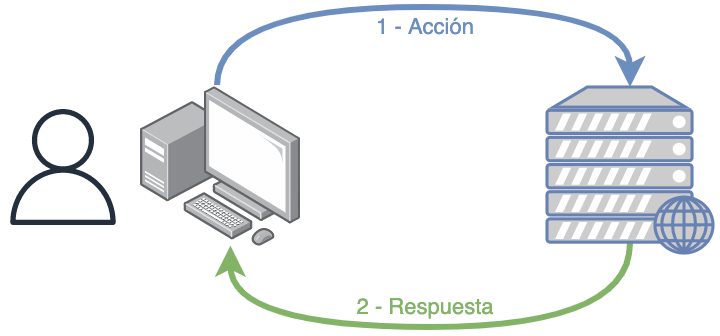
\includegraphics[width=0.7\linewidth]{ejecucion_remota.png}
\end{center}

Hoy en día es muy habitual este tipo de sistemas a través de disintos \textbf{CLI} (\textit{client line interface})  o \textbf{GUI} (\textit{graphic user interface}) que nos permiten administrar servicios remotos. Por ejemplo:

\begin{itemize}
    \item \textbf{{https://www.mysql.com/}{MySQL}}: El sistema gestor de base de datos \href{https://www.mysql.com/}{MySQL} cuenta con un cliente para realizar la  conexión, ya sea desde el propio equipo o desde un equipo remoto.

    Este cliente se puede ejecutar desde línea de comandos, aunque también viene integrado en distintos interfaces gráficos como \href{https://dev.mysql.com/downloads/benchmarks.html}{MySQL Benchmark}, \href{https://dbeaver.io/}{Dbeaver}, ...

    \item \textbf{\href{https://aws.amazon.com/es/cli/}{AWS CLI}}: Es el interfaz de línea de comandos para poder administrar de manera remota los servicios contratados en la nube AWS de Amazon.

    \item \textbf{\href{https://cloud.google.com/cli}{Gcloud CLI}}: Similar al caso anterior pero esta vez para Google Cloud.

    \item \textbf{\href{https://www.microsoft.com/en-us/download/details.aspx?id=45520}{Remote Server Administration Tools for Windows 10}}: En este caso se trata de un interfaz gráfico (\textbf{GUI}) que nos permite administrar un Windows Server desde un equipo Windows 10.
\end{itemize}


Antes de poder realizar la conexión remota con el cliente \textbf{debemos configurar un sistema de autenticación} para que el servicio remoto acepte las peticiones enviadas. En algunos casos será usando unos sistemas de certificados y en otros introduciendo un usuario y contraseña que establecerá una sesión temporal.

En el caso de AWScli y GCloud no nos estamos conectando directamente a nuestros servidores alojados en esas nubes, si no que lanzamos la orden a un “proxy” que verificará nuestros credenciales, verá los permisos que tenemos y después realizará la acción solicitada.


%TODO: mirar algo de esto
%COSAS A MIRAR:
%
%
%ADmin center
%
%https://learn.microsoft.com/en-us/windows-server/manage/windows-admin-center/plan/installation-options
%
%sconfig en windows    https://learn.microsoft.com/en-us/windows-server/administration/server-core/server-core-sconfig
%
%
%diferencias entre windows server core and escritorio https://learn.microsoft.com/en-us/windows-server/get-started/install-options-server-core-desktop-experience


\section{Acceso remoto}
Este sistema permite acceder al sistema y podremos administrarlo como si nos encontrásemos delante. Dependiendo del sistema la conexión nos permitirá interactuar de alguna de las siguientes maneras:

\begin{itemize}
    \item \textbf{CLI}: Mediante una conexión de línea de comandos. Es el caso más habitual en servidores GNU/Linux y la conexión se hace a través del protocolo seguro \textbf{SSH}.

    \item \textbf{GUI}: Podremos obtener un interfaz gráfico con el que veremos lo que está ocurriendo en pantalla en ese momento. En este caso, dependiendo del sistema, existirán distintas opciones, pero vamos a nombrar dos de ellas:

    \begin{itemize}
        \item \textbf{RDP}: Es el protocolo de escritorio remoto de Microsoft que transmite la información gráfica que el usuario debería ver por la pantalla, la transforma en el formato propio del protocolo, y la envía al cliente conectado. El problema es que este sistema desconecta al usuario que está logueado para poder hacer uso del escritorio remoto.

        \item \textbf{VNC}: En inglés \textit{Virtual Network Computing}, es un servicio con estructura \textbf{cliente-servidor} que permite visualizar el escritorio del servidor desde un programa cliente. En este caso, no existe desconexión del usuario que está logueado y por tanto podrá ver lo que le están realizando de manera remota.

        Es muy habitual que los equipos de usuarios ya tengan la instalación del servidor hecha, para que de esta manera, en caso de incidencia, poder realizar la conexión remota sin que el usuario tenga que realizar ninguna acción.
    \end{itemize}
\end{itemize}

A continuación se va a detallar algunos de los métodos mencionados.



\section{SSH}
SSH es un protocolo de comunicación segura mediante cifrado cuya función principal es el acceso remoto a un servidor. La arquitectura que utiliza es la de cliente-servidor.

Aunque el uso más habitual de SSH es el acceso remoto, también se puede utilizar para:
\begin{itemize}
    \item Securizar protocolos no seguros mediante la realización de túneles.
    \item Acceder a un equipo saltando a través de otro.
\end{itemize}

Estas funcionalidades las veremos más adelante.


\subsection{Servidor SSH}
En el servidor al que nos queramos conectar deberá estar instalado el demonio/servicio SSH, conocido como \textbf{sshd}. Es habitual que ya esté instalado en sistemas GNU/Linux, pero de no ser así deberemos usar el sistema de paquetes de nuestra distribución para hacer la instalación. El nombre suele ser \textbf{openssh-server}.

Este servicio por defecto se pondrá a la escucha en el puerto 22/TCP:

\begin{mycode}{SSHd escuchando en puerto 22}{console}{{\scriptsize }}
ruben@vega:~$ sudo ss -pntaln
State   Recv-Q   Send-Q   Local Address:Port   Peer Address:Port   Process
LISTEN  0        128      0.0.0.0:22           0.0.0.0:*           users:(("sshd",pid=1122,fd=3))
LISTEN  0        128      [::]:22              [::]:*              users:(("sshd",pid=1122,fd=4))
\end{mycode}

La configuración del servicio se realiza a través de un fichero de configuración que está situado en la ruta \configfile{/etc/ssh/sshd_config}. Las distribuciones de GNU/Linux ya traen una configuración predeterminada que suele constar de las siguientes directivas (aunque hay muchas más):

\begin{itemize}
    \item \textbf{Port}: Normalmente viene comentada, ya que el puerto por defecto es el 22. En caso de querer cambiar el puerto, podremos modificar esta línea, asegurando que no esté comentada.

    \item \textbf{ListenAddress}: Por defecto SSH se pondrá a la escucha en todos los interfaces que tengamos configurados. Si sólo nos interesa escuchar en alguna de las IPs que tengamos configuradas, deberemos modificar esta configuración.

    \item \textbf{PermitRootLogin}: Para evitar problemas de seguridad, esta directiva suele estar configurada a “\textbf{No}”, para evitar que se puedan usar los credenciales de root para hacer el login.

    \item \textbf{PubkeyAuthentication}: Esta directiva permite realizar la conexión a través de unas claves públicas/privadas que podemos crear. Se explicará más adelante.
\end{itemize}

Hoy día también se puede instalar en Windows 10 y posteriores a través de un comando, siendo administrador de PowerShell:

\begin{mycode}{Instalando OpenSSH Server en Windows 10}{powershell}{{\footnotesize }}
PS C:\Windows\System32> Add-WindowsCapability -Online -Name OpenSSH.Server~~~~0.0.1.0

PS C:\Windows\System32> Start-Service sshd

PS C:\Windows\System32> Set-Service -Name sshd -StartupType 'Automatic'
\end{mycode}

O desde el interfaz gráfico a través de las “\textbf{Características opcionales}”, buscando por ssh
\begin{center}
    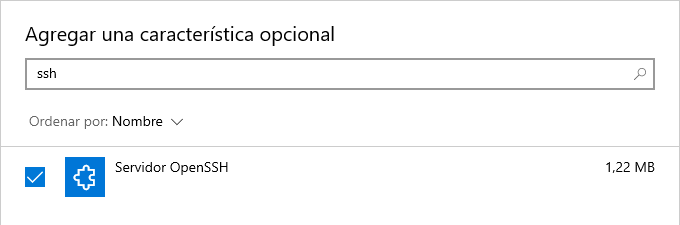
\includegraphics[frame,width=0.6\linewidth]{ssh_server_windows.png}
\end{center}


\subsection{Cliente SSH}
El cliente SSH es aquel programa que a través del protocolo SSH se puede conectar a un servidor SSH. Existen distintos tipos de clientes que podemos utilizar:

\begin{itemize}
    \item \textbf{CLI}: El cliente de consola es el más habitual. Está instalado de forma habitual en todas las distribuciones de GNU/Linux (normalmente el paquete se llama \textbf{openssh-client}). También lo encontramos instalado por defecto en MacOS.

    Hoy día también está instalado en Windows 10, y de no estar, se puede instalar a través de las “\textbf{Características Opcionales}”.

    \item \textbf{GUI}: Existen distintos interfaces gráficos que nos puede interesar utilizar:
    \begin{itemize}
        \item \textbf{\href{https://putty.org/}{Putty}}: Un cliente muy habitual en entornos Windows.
        \item \textbf{\href{https://github.com/cyd01/KiTTY/}{Kitty}}: Una versión mejorada del anterior.
        \item \textbf{\href{https://www.termius.com/}{Termius}}: Cuenta con versión de escritorio y móvil.
    \end{itemize}
\end{itemize}


Para realizar la conexión al servidor SSH debemos conocer:

\begin{itemize}
    \item \textbf{Dirección del servidor}: Ya sea mediante IP o nombre FQDN (\textit{fully qualified domain name}) que se resuelva.
    \item \textbf{Puerto}: Ya hemos comentado que por defecto el puerto es 22.
    \item \textbf{Usuario}: Para realizar el sistema de autenticación, necesitamos un usuario que exista en el sistema.
    \item \textbf{Contraseña}: Los credenciales de acceso del usuario.
\end{itemize}

Para realizar la conexión desde un cliente de consola ejecutaremos:

\begin{mycode}{Conexión SSH }{console}{ }
ruben@vega:~$  ssh usuario@192.168.1.200 -p 22
\end{mycode}

En el comando anterior podemos identificar:
\begin{itemize}
    \item \textbf{ssh}: el cliente de consola
    \item \textbf{usuario}: el nombre del usuario con el que nos queremos conectar al servidor remoto.
    \item \textbf{@}: la arroba en inglés significa “at”, que indica “usuario en el servidor X”.
    \item \textbf{192.168.1.200}: La IP del servidor al que nos queremos conectar.
    \item \textbf{-p 22}: Estos dos parámetros van juntos,  “-p” indica que vamos a indicar el puerto de conexión y “22” que nos queremos conectar a ese puerto. Debido a que 22 es el puerto por defecto, podríamos no poner estas opciones si sabemos que el servidor escucha en el puerto 22.
\end{itemize}

Si realizamos la conexión a través de un cliente de interfaz, como es putty, el aspecto será el siguiente, donde sólo podremos introducir la IP del servidor. Cuando se comience con la conexión nos pedirá los credenciales de acceso.

\begin{center}
    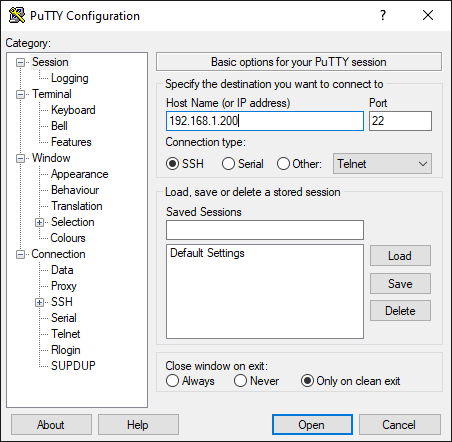
\includegraphics[width=0.5\linewidth]{putty.png}
\end{center}


Si es la primera vez que nos conectamos a un servidor mediante SSH nos saldrá un mensaje como el siguiente:

\begin{mycode}{Conexión SSH }{console}{{\small }}
ruben@vega:~$  ssh usuario@192.168.1.200 -p 22

The authenticity of host '192.168.1.200 (192.168.1.200)' can't be established.
ECDSA key fingerprint is SHA256:uK9MOl0gLDhTtCrlcafc1zVObVA/vnOMn6TWFsQb23o.
Are you sure you want to continue connecting (yes/no/[fingerprint])?
\end{mycode}

Este “key fingerprint” es un identificador que está relacionado con el fichero de “\textbf{clave pública}” del servidor. Es como el DNI del servidor. La primera vez se nos guarda ese \textit{fingerprint}, y en caso de que en una próxima conexión varíe, nos avisará. No suele ser habitual que este identificador cambie.


\hypertarget{ssh_clave_publica_privada}{}
\subsection{Conexión mediante certificados de clave pública/clave privada}

Existe una alternativa a la hora de realizar una conexión SSH para que no nos pida la contraseña del usuario, y es \textbf{hacer uso de los certificados de clave pública y clave privada}. Este concepto de “clave pública y clave privada” viene de la \href{https://es.wikipedia.org/wiki/Criptograf%C3%ADa_asim%C3%A9trica}{\textbf{criptografía asimétrica}}.

Este sistema de criptografía asimétrica hace uso de dos claves que están asociadas entre sí:
\begin{itemize}
    \item \textbf{Clave privada}: Es la base del sistema criptográfico, y como su nombre indica, se debe de mantener en privado. \textbf{Nunca se debe de compartir}, ya que entonces se podrían hacer pasar por nosotros.
    \item \textbf{Clave pública}: Asociada a la clave privada, la clave pública puede ser compartida y enviada a otros ordenadores para poder realizar la conexión.
\end{itemize}

Para generar el par de claves se realiza con el siguiente comando:

\begin{mycode}{Crear par de claves pública/privada}{console}{}
ruben@vega:~$  ssh-keygen
Generating public/private rsa key pair.
Enter file in which to save the key (/home/ruben/.ssh/id_rsa):

Enter passphrase (empty for no passphrase):
Enter same passphrase again:

Your identification has been saved in /home/ruben/.ssh/id_rsa
Your public key has been saved in /home/ruben/.ssh/id_rsa.pub
The key fingerprint is:
SHA256:SPqPOYBmPb8PCFhcZgqcWZPZzaL5RNfMeKmHqebvC7E ruben@vega
The key's randomart image is:
+---[RSA 3072]----+
|o +oB o = .      |
| * B.+ = *       |
|  + + + =        |
| o o + = .       |
|. .o+.o S        |
|  +.+*o          |
| o  +Eo          |
|     .+=         |
|      *B+        |
+----[SHA256]-----+
\end{mycode}

El comando muestra los siguientes pasos:
\begin{enumerate}
    \item Creación de la pareja de claves pública/privada haciendo uso del sistema criptográfico \href{https://en.wikipedia.org/wiki/RSA_(cryptosystem)}{\textbf{RSA}}.
    \item Lugar donde se va a guardar la clave privada. Por defecto en \configdir{~/.ssh/id_rsa}.
    \item Contraseña para securizar la clave privada. De esta manera, para poder usarla habrá que introducir dicha contraseña. Dado que nosotros queremos evitar introducir contraseñas, lo dejaremos en blanco.
    \item Lugar donde se va a guardar la clave pública. Por defecto en \configdir{~/.ssh/id_rsa.pub}
\end{enumerate}

Una vez tenemos nuestro par de claves, podemos copiar la clave pública al usuario del servidor que nos interese mediante el siguiente comando:

\begin{mycode}{Crear par de claves pública/privada}{console}{}
ruben@vega:~$  ssh-copy-id user@servidor_remoto
\end{mycode}

Para ello es imprescindible conocer previamente la contraseña del usuario en el servidor. El comando \commandbox{ssh-copy-id} realizará una conexión SSH y copiará el contenido de la \textbf{clave pública}, \configdir{~/.ssh/id_rsa.pub}, dentro del fichero \configfile{~/.ssh/authorized_keys} del usuario en el servidor remoto. Este paso se puede realizar a mano (con un editor de texto).

\errorbox{\textbf{Windows no tiene el comando “ssh-copy-id”, por lo que deberemos hacer el paso a mano, tal como se ha explicado.}}

Al realizar la siguiente conexión, ya no necesitaremos introducir la contraseña del usuario, ya que el sistema remoto podrá autenticarnos a través del sistema clave pública/privada.


\subsection{Crear túneles SSH}
Una de las funcionalidades extra de SSH es la posibilidad de crear “túneles” para securizar protocolos no seguros, o poder acceder a servicios que sólo escuchan en \textit{localhost}.

Pongamos como ejemplo el siguiente escenario:

\vspace{-15pt}
\begin{center}
    
\includegraphics[width=0.5\linewidth]{tunel1.png}
\end{center}
\vspace{-15pt}

Tenemos un servidor web con Apache y MySQL al que queremos acceder. Por seguridad MySQL \textbf{sólo está escuchando en localhost (127.0.0.1)}, por lo que el acceso al servicio MySQL no es posible. Para administrarlo nos tenemos que conectar al servidor, y realizarlo de manera local.

En este punto es donde entra en juego la creación de un túnel seguro al servidor, para poder acceder al servicio remoto. \textbf{Para ello es imprescindible poder realizar una conexión SSH} (ya sea mediante usuario o clave pública/privada).

Para crear un túnel, desde el equipo de escritorio, lanzaremos el siguiente comando:

\begin{mycode}{Crear par de claves pública/privada}{console}{}
ruben@vega:~$  ssh usuario@192.168.1.200 -L 6306:127.0.0.1:3306 -N
\end{mycode}

Al ejecutar este comando, habremos creado un túnel que enlaza el puerto remoto 3306 (que sólo se escucha en el “127.0.0.1” del servidor), con el puerto local 6306 del equipo de escritorio. A continuación la explicación del comando y sus parámetros:


\begin{itemize}
    \item “\textbf{ssh usuario@192.168.1.200}”: es como una conexión SSH normal. Lo que estamos indicando es que queremos conectarnos con  “usuario” al servidor remoto 192.168.1.200 a través de SSH.
    \item \textbf{-L 6306:127.0.0.1:3306}: Especifica que el puerto local especificado se va redirigir al puerto e IP remota. Para entender esto hay que separar dos partes de los parámetros:
    \begin{itemize}
        \item \textbf{6306}: Especifica la IP y el puerto local. En este caso, antes del puerto no hemos especificado IP, por lo que se creará un puerto 6306 que sólo se pone a la escucha en \textbf{\textit{localhost}} en el equipo de escritorio
        \item \textbf{127.0.0.1:3306}: Esta es la dirección y puerto remoto al que nos queremos conectar. En este caso, es el puerto 3306 que está escuchando en la IP 127.0.0.1 del servidor.
    \end{itemize}
    \item \textbf{-N}: Sirve para que no ejecute ningún comando en el servidor remoto, y por tanto no nos abrirá conexión de terminal.
\end{itemize}

A nivel visual, y para entender de mejor manera lo realizado, sirva la siguiente imagen y los pasos que se pueden dar en un escenario real:

\vspace{-10pt}
\begin{center}
    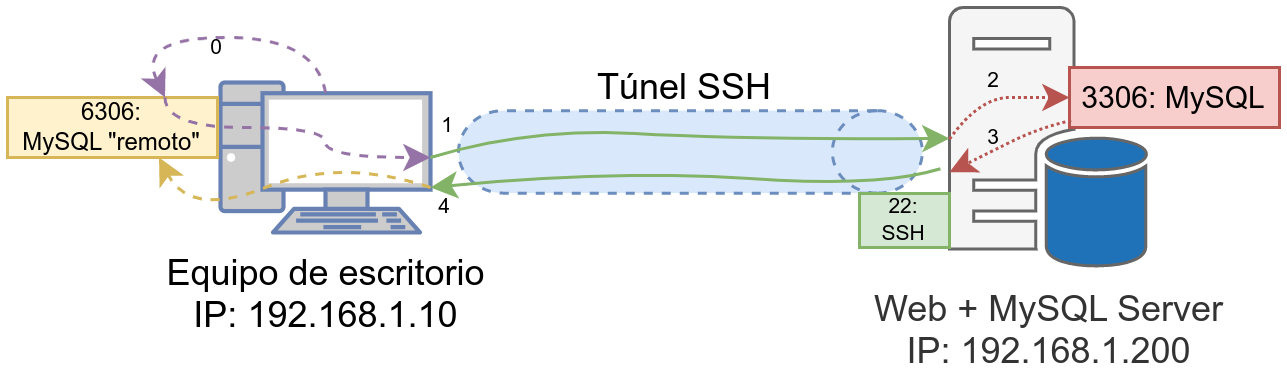
\includegraphics[width=\linewidth]{tunel2.png}
\end{center}
\vspace{-10pt}

Con una aplicación en el equipo de escritorio queremos conectarnos al servidor MySQL que sólo escucha en el servidor remoto. Ejecutamos el túnel visto anteriormente, y los pasos que podremos realizar son los siguientes:

\begin{enumerate}
    \item[0.] Mediante una aplicación nos podemos conectar al puerto local 6306, que ha sido creado mediante el comando anterior. Este puerto local está redirigido al puerto del servidor remoto. Por lo tanto la conexión  se securiza a través del túnel
    \item Como el túnel está establecido, la conexión viaja de manera segura a través de él.
    \item Al llegar al servidor remoto, sabe que la conexión debe ir al puerto 3306 de la IP 127.0.0.1, que es lo establecido en el comando.
    \item La conexión vuelve al túnel.
    \item Viaja por el túnel hasta llegar a la comunicación que se había establecido previamente.
\end{enumerate}

De esta manera, hemos podido realizar una conexión a un servicio remoto a través de SSH y completamente seguro.


\subsubsection{Acceder a un equipo saltando a través de otro.}
Este es un caso especial de túnel, similar a lo explicado previamente. En lugar de querer realizar una conexión a un servicio del equipo al que nos conectamos, en este caso lo usaremos de salto para acceder a otro servidor.

\vspace{-10pt}
\begin{center}
    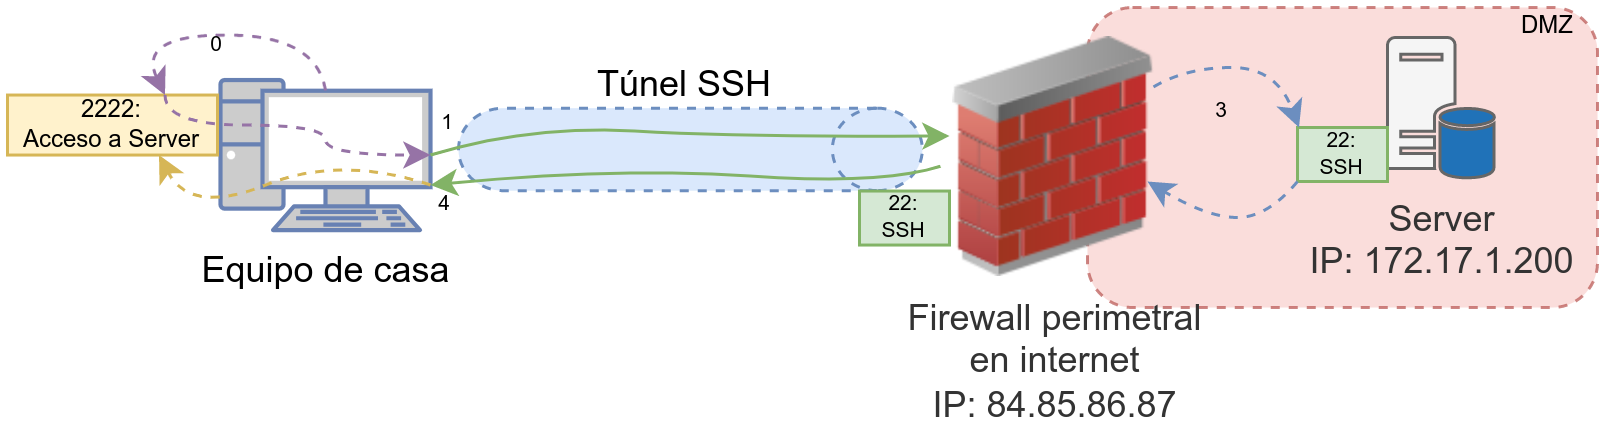
\includegraphics[width=\linewidth]{tunel3.png}
\end{center}
\vspace{-10pt}

En este caso estando en casa nos queremos conectar a un equipo de la oficina. No tenemos VPN, y no hay redirección de puertos directa, pero podemos acceder al firewall perimetral. Por lo tanto, lo podemos utilizar para saltar al servidor que nos interesa.

En este caso, el comando a ejecutar sería:

\begin{mycode}{Crear par de claves pública/privada}{console}{{\small}}
ruben@vega:~$  ssh usuario_firewall@84.85.86.87 -L 2222:172.17.1.200:22 -N
\end{mycode}

De esta manera, ahora desde nuestro equipo podremos realizar una conexión SSH al puerto 2222 que realmente será una redirección que viaja a través del túnel hasta el firewall, y que a su vez redirige al puerto 22 del servidor 172.17.1.200.

\warnbox{\textbf{El servicio remoto al que nos queremos conectar debe escuchar en la IP del equipo al que nos queremos conectar. El equipo que usamos para saltar debe poder conectarse a él.}}


%\section{VNC}

% TODO: comentar VNC




\clearpage